\chapter{Proposed System}
\label{ch:Proposed System}
Emotion detection from text has now become one of the key feature to understand peoples emotion. Everyone writes about their feelings or emotion in their social media, comment box or in inbox. If a system can identify those emotions from texts then it will be very help full to understand the people's thoughts. For this reason we build a system that can detect emotion from text. In this chapter we represents our architectural diagram and detailed module design of our text based emotion detection system.

\section{Design}
Here we represent the architectural design of the system. In our system we use text data from different anonymous chat data. The chat data is in text format. Data already includes different emotions specified. Then this data are sent to the finale stage where the emotion is analysed using LSTM network architecture.


\section{Module Description}
Here we provide detailed information about the modules of our system. That defines how our system works.
\begin{itemize}
\item Data collection
\item Data Preprocessing
\item Glove Embedding Vector Model
\item LSTM
\end{itemize}

\subsection{Data Collection}
To run the system at first we need a data set from where we can perform emotion detection. For our system, dataset was collected from kaggle.com. It contains about 20000 anonymous chat data from different whatsapp groups. The entire dataset is divided into three parts for testing, training and validation. The train dataset contains 16000 text data and test and validation dataset contains 2000 text data each.

\subsection{Data Preprocessing}
Preprocessing involves removing garbage value or noise from dataset. There's possibility of irrelevant data presence in dataset which are not necessary and therefore discarding them would benefit the model's training capacity and overall accuracy in the end. In our textual dataset, preprocessing involved turning all upper case letters in lower case letters, removing stop signs like full stop, coma and question mark signs.   

\subsection{Glove Embedding Vector Model}
GloVe, short for Global Vectors for Word Representation, is an unsupervised learning algorithm for obtaining vector representations (embeddings) of words.GloVe constructs a global word-word co-occurrence matrix from large text corpora and then factorizes it to capture the semantic relationships between words. The resulting embeddings encode meaningful semantic relationships and are widely used in natural language processing tasks such as text classification and sentiment analysis. GloVe embeddings are pretrained on extensive datasets, making them effective for capturing nuanced language patterns and aiding in tasks where understanding the context and meaning of words is crucial~\cite{ref10}.

\subsection{LSTM}
LSTM stands for long short-term memory networks which is used in the field of Deep Learning.LSTM is a advanced version of recurrent neural networks (RNNs) that is design to learn long-term dependencies, especially in sequence prediction problems.

\subsubsection{Architecture of LSTM}
The role of an LSTM model is held by a memory cell known as a cell state that maintains its state over time. The cell state is the horizontal line that runs through the top of the below diagram. Information can be added to or removed from the cell state in LSTM and is regulated by gates. These gates optionally let the information flow in and out of the cell. It contains a point-wise multiplication operation and a sigmoid neural net layer that assist the mechanism. The sigmoid layer gives out numbers between zero and one, where zero means nothing should be let through, and one means everything should be let through.~\cite{ref9}


\begin{figure}[ht!]
  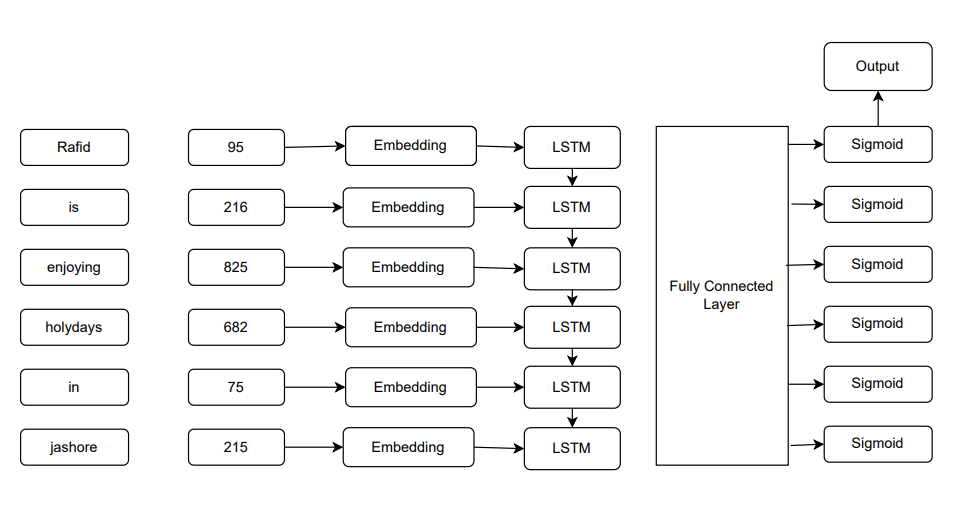
\includegraphics[width=\linewidth]{chapters/LSTM.png}
  \caption{LSTM architecture}
\end{figure}

There are mainly five layers in LSTM network. But layer an be added to improve the accuracy of the model. The five layers are:
\begin{itemize}
\item \textbf{Embedding Layer:} This Layer is responsible for converting word tokens into embedding of a specific size like 256, 512 etc. This layer maps a sequence of word indices to embedding vectors and learns the word embedding during training.
In this layer the word tokens are converted into embedding of a specific size like 256,512 etc. This layer also responsible for mapping a sequence of word indices to embedding vectors and learns the word embedding during training.

\item \textbf{LSTM Layer:}This layer sequentially process data and keep its hidden state through time. It keeps previous memory and process with current memory and decides whether to keep current memory or remain with old memory.
   
\item \textbf{Fully Connected Layer:} This layer indicates those layers where all inputs from one layer are connected to every unit of the next layer.

\item \textbf{Sigmoid Activation Layer:} This layer is responsible for converting all output values in the range of 0 to 1. It means it can either let no flow or complete flow of information throughout the gates.

\item \textbf{Output Layer:} Output layer is the final layer of the architecture. This layer is responsible for generating output which is obtained from sigmoid layer. The output formate is 2d array of real numbers where the first dimension indicates the number of samples given to the LSTM layer and second dimension is the dimensionality of the output space defined by the units
parameter in Keras LSTM implementation.
\end{itemize}






























